\section{Non solo cloud}\label{sec:mooncloud-not-only-cloud}
MoonCloud è stata progettata per poter essere eseguita sul cloud, e, più di tutto,
la si vuole \textit{as-a-service}\footnote{L'ultimo capitolo è dedicato ad ulteriori
evoluzioni dell'architettura MoonCloud}, ciò significa che i clienti che vogliono
certificare parte della propria infrastruttura cloud, non devono installare alcun
software, semplicemente usano la \texttt{Dashboard} per regolare i controlli
che vogliono fare.

La verifica del fatto che, ad esempio, si utilizzi uno storage cifrato, può essere
effettuata mediante hook messi a disposizione dal cloud provider.

Tuttavia, si è voluto ampliare la platea di possibili target per MoonCloud:
si supponga che anziché voler analizzare la configurazione di OpenStack di
un deployment pubblico si vogliano verificare che certe policy di \texttt{Active
Directory} all'interno di una rete aziendale.
Anziché utilizzare gli hook messi a disposizione da un cloud provider, occorrerebbe
utilizzare le API di \texttt{Active Directory}, e come veicolo di accesso ad esse
non più (ad esempio) HTTP, ma bisognerebbe aver accesso alla rete interna
in cui Windows Server è in esecuzione.
Infatti, l'obiettivo di MoonCloud per espandere i propri clienti è quello di non
solo essere in grado di analizzare dei target nel cloud, ma anche in una rete
aziendale fisica.
Ciò pone un grande problema: l'accesso alla rete fisica, infatti non si potrebbero
più utilizzare gli hook forniti dal cloud provider.

A maggior ragione, il problema si fa più complesso se si vogliono verificare
proprietà relative a servizi \textit{solo interni} di una rete, che non sono
esposti all'esterno.

Occorre quindi cambiare ``trasporto'', e trovare un modo per avere accesso
\textit{dall'interno}, visto che tali reti interne (definite \textit{reti target})
sono ragionevolmente e auspicabilmente protette da un firewall.

Nella fattispecie, si è investigato l'utilizzo di una soluzione basata su VPN,
per la quale si porta fisicamente nella rete target un VPN client, responsabile
di connettersi alla rete MoonCloud e di fornire un canale di comunicazione
altamente sicuro.
Le Docker machine restano deployate nel cloud in cui MoonCloud stessa è, e le
loro richieste di analisi passano tramite la VPN.
Questo è stato infatti argomento della prima e più complessa parte della mia tesi.

Sono stati definiti i seguenti requisiti:
\begin{itemize}
    \item soluzione altamente sicura
    \item se possibile, basata su TLS/HTTPS. Questo perché si ritiene che
    almeno il traffico HTTP ed HTTPS sia consentito anche dai firewall
    più stringenti. Una VPN basata su TLS quindi è ragionevolmente consentita
    senza necessità di riconfigurare il firewall aziendale.
    Questo si è anche tradotto in una preferenza di TCP rispetto ad UDP.
    \item Preferire VPN configurabili e flessibili rispetto a
    VPN performanti ma poco adattibili ai requisiti.
    \item La soluzione VPN deve essere il più possibile lightweight
    per la rete target, ovvero deve poter, nei limiti del
    possibile, funzionare senza dover configurare nulla nella rete
    target (ad eccezione del VPN client stesso).
\end{itemize}

\begin{figure}
    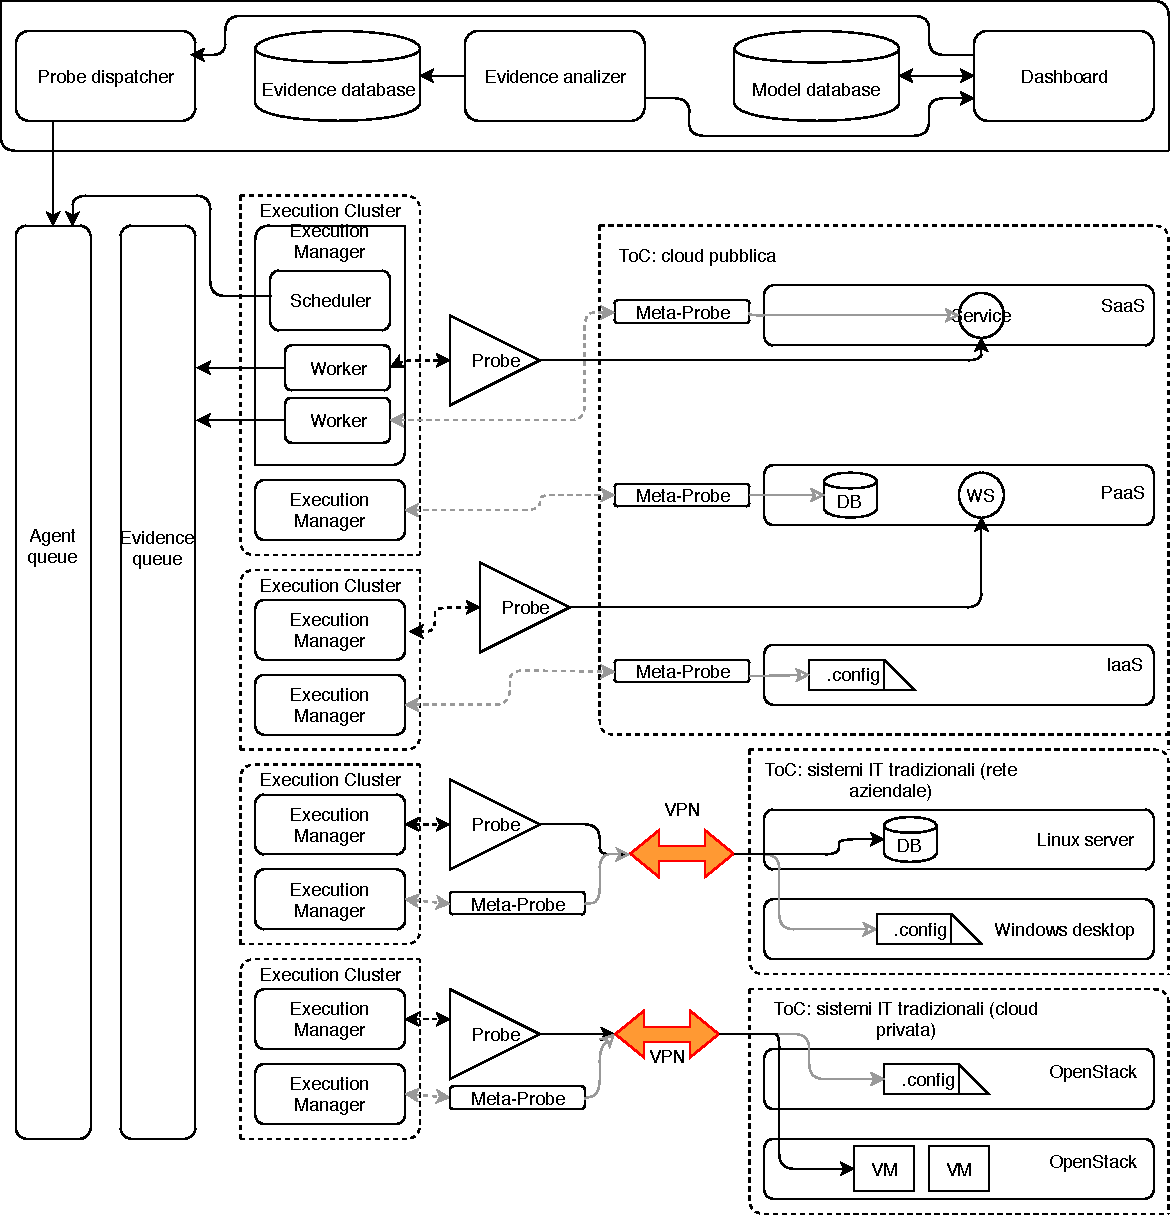
\includegraphics[scale=0.6]{img/mooncloud_archi_extended}
    \label{fig:mooncloud-archi-extended}
    \caption[L'architettura con l'utilizzo di una VPN per
    consentire l'analisi di sistemi IT tradizionali]
    {L'architettura con l'utilizzo di una VPN}
\end{figure}